\documentclass[a4paper, 12pt]{article}%тип документа

%отступы
\usepackage[left=2cm,right=2cm,top=2cm,bottom=3cm,bindingoffset=0cm]{geometry}

%Русский язык
\usepackage[T2A]{fontenc} %кодировка
\usepackage[utf8]{inputenc} %кодировка исходного кода
\usepackage[english,russian]{babel} %локализация и переносы

%Вставка картинок
\usepackage{wrapfig}
\usepackage{graphicx}
\graphicspath{{pictures/}}
\DeclareGraphicsExtensions{.pdf,.png,.jpg}

%Графики
\usepackage{multirow}
\usepackage{pgfplots}
\usepackage{rotating}
\usepackage{pgfplotstable}
\usepackage{booktabs}
\usepackage{multirow}
\pgfplotsset{compat=1.9}

%Математика
\usepackage{amsmath, amsfonts, amssymb, amsthm, mathtools}

%Заголовок
\author{Сифат Мд Абдуллах Ал Хасиб \\
Физтех школа электроники, фотоники и молекулярной физики \\
Группа Б04-105}
\title{\textbf{Лаборатория Работа 2.3.1 \\ 
Получение и измерение вакуума}}
\begin{document}
\maketitle
\section{Введение}\textbf{Цель работы:} 1) измеренеи объёмов форвакуумной и высоковакуумной частей установки; 2) определение скорости откачки системы в стационарном режиме, а также по ухудшению и по улучшению вакуума. \\
\textbf{В работе используется:} вакуумная установка с манометрами: масляным, термопарным и ионизационным. По степени разряжения вакуумные установки принято делить на три класса: 1) низковакуумные -- до $10^{-2}$-$10^{-3}$ торр; 2) высоковакуумные -- $10^{-4}$-$10^{-7}$ торр; 3) установки сверхвысокого вакуума -- $10^{-8}$-$10^{-11}$ торр. С физической точки зрения низкий вакуум переходит в высокий, когда длина свободного пробега молекул газа оказывается сравнима с размерами установки; сверхвысокий вакуум характерен крайней важностью процессов адсорбции частиц на поверхности вакуумной камеры.
\section{Теоретическая справка} 
\subsection{Процесс откачки}
	Производительность насоса определяется скоростью откачки $W$ (л/с): $W$ — это объем газа, удаляемого из сосуда при данном давлении за единицу времени. Скорость откачки форвакуумного насоса равна емкости воздухозаборной камеры, умноженной на число оборотов в секунду.
Рассмотрим обычную схему откачки. Разделим вакуумную систему на две части: «откачиваемый объем» (в состав которого включим используемые для работы части установки) и «насос», к которому, кроме самого насоса, отнесем трубопроводы и краны, через которые
производится откачка нашего объема. Обозначим через $Q_d$ количество газа, десорбирующегося с поверхности откачиваемого объема в единицу времени, через $Q_i$ — количество газа, проникающего в единицу времени в этот объем извне — через течи. Будем считать, что насос обладает скоростью откачки $W$ и в то же время сам является источником газа; пусть $Q_n$ — поток газа, поступающего из насоса назад в откачиваемую систему. Будем измерять количество газа $Q_d$, $Q_i$ и $Q_n$ в единицах $PV$ (легко видеть, что это произведение с точностью до множителя $RT/ \mu$ равно массе газа). Основное уравнение, описывающее процесс откачки, имеет вид

\begin{equation}
\label{otkachka}
	-VdP=(PW-Q_d-Q_n-Q_i)dt.
\end{equation}

Левая часть этого уравнения равна убыли газа в откачиваемом объеме $V$ , а правая определяет количество газа, уносимого насосом, и количество прибывающего вследствие перечисленных выше причин
за время $dt$. При достижении предельного вакуума (давление $P_{pr}$)

\begin{equation}
\label{predel_1}
	\frac{dP}{dt}=0,
\end{equation}

\begin{equation}
\label{predel_2}
	W=\frac{\sum Q_i}{P_{pr}}.
\end{equation}

Обычно $Q_i$ постоянно, a $Q_n$ и $Q_d$ слабо зависят от времени, поэтому в наших условиях все эти члены можно считать постоянными. Считая также постоянной скорость откачки $W$ , уравнение~(\ref{otkachka}) можно проинтегрировать и, используя~(\ref{predel_1}), получить
\begin{equation}
\label{davlenie}
	P = P_o \exp{(-\frac{W}{V} t)} + P_{pr}.
\end{equation}


\subsection{Течение газа через трубу}
	Характер течения газа существенно зависит от соотношения между размерами системы и длиной свободного пробега молекул. При атмосферном давлении и даже при понижении давления до форвакуумного длина свободного пробега меньше диаметра трубок и течение откачиваемого газа определяется его вязкостью, т. е. взаимодействием его молекул. При переходе к высокому вакууму картина меняется. Столкновения молекул между собой начинают играть меньшую роль, чем соударения со стенками. Течение газа в трубе напоминает в этих условиях диффузию газа из области больших концентраций в области, где концентрация ниже, причем роль длины свободного пробега играет ширина трубы.
Для количества газa, протекающего через трубу в условиях высокого вакуума или, как говорят, в кнудсеновском режиме, справедлива формула

\begin{equation}
\label{formula}
	\frac{d(PV)}{dt}=\frac{4}{3}r^3 \sqrt{\frac{2\pi RT}{\mu}} \frac{P_2-P_1}{L}.
\end{equation}
Применим эту формулу к случаю, когда труба соединяет установку с насосом.
Пренебрежем давлением $P_1$ у конца, обращенного к насосу. Будем измерять количество газа, покидающего установку при давлении $P = P_2$. Пропускная способность трубы

\begin{equation}
	C_{tr}=(\frac{dV}{dt})_{tr}=\frac{4}{3}\frac{r^3}{L}\sqrt{\frac{2\pi RT}{\mu}}.
\end{equation}

	Мы видим, что пропускная способность зависит от радиуса трубы в третьей степени и обратно пропорциональна ее длине. В вакуумных установках следует поэтому применять широкие короткие  трубы.
	
	При расчете вакуумных систем нужно принимать во внимание также пропускную способность отверстий, например, в кранах. Для диффузионного насоса можно считать, что каждая молекула воздуха, попавшая в кольцевой зазор между соплом и стенками насоса, увлекается струей пара и не возвращается обратно в откачиваемый объем. Скорость откачки такого насоса можно считать равной пропускной способности отверстия с площадью, равной площади кольцевого зазора, т. е. насос качает как кольцевой зазор, с одной стороны которого расположен откачиваемый объем, а с другой -- пустота.
\section{Модель экспермиента}
\begin{enumerate}
\item
	Определим объемы форвакуумной и высоковакуумной частей установки. Сначала впустим атмосферу в установку. Запрем воздух при комнатных условиях в капилляре между кранами 5 и 6. После этого откачаем воздух из оставшейся части установки (сделав это в два этапа - сначала насос должен откачать сам себя, а только потом - установку). После этого мы сначала высвободим запертый воздух только в ФВ часть, а затем добавим к ней и ВВ. Тогда записав уравнение Менделеева-Клапейрона и зная объем капилляра, мы найдем объемы соответствующих частей установки:
\begin{equation}
	P_0 V_0 = P_v (V_f + V_v),
\end{equation}
где $P_0$ -- атмосферное давление; $V_0$ -- объем капилляра и кранов 5 и 6; $P_v$ -- установившееся давление; $V_f$ и $V_v$ -- соотвественно объемы форвауумной и высоковакуумной частей.
	
\item
	Для измерения скорости откачки диффузионного насоса измерим улучшение вакуума во времени. Построим график зависимости $-\ln{\frac{P-P_{pr}}{P_0}}$ от $t$. Из формулы~(\ref{davlenie}) следует, что наклон, построенной кривой, есть $W / V$

\item
	Откроем кран 6 и создадим исскуственную течь через капилляр. Рассчитаем производительность насоса по различию $P_{pr}$ и $P_u$, где $P_u$ -- установившееся давление в высоковакуумной части с искусственной течью. В условиях высокого вакуума справдлива формула~(\ref{formula}), где положим $P_1 := P_u$, $P_2$ -- давление в форвакуумной части. 


\end{enumerate}
\section{Ход работы}
\subsection{Рассчет скорости откачки}
Построим график зависимости давления от времени при открытом кране 3, что соответсвует улучшению вакуума: \\
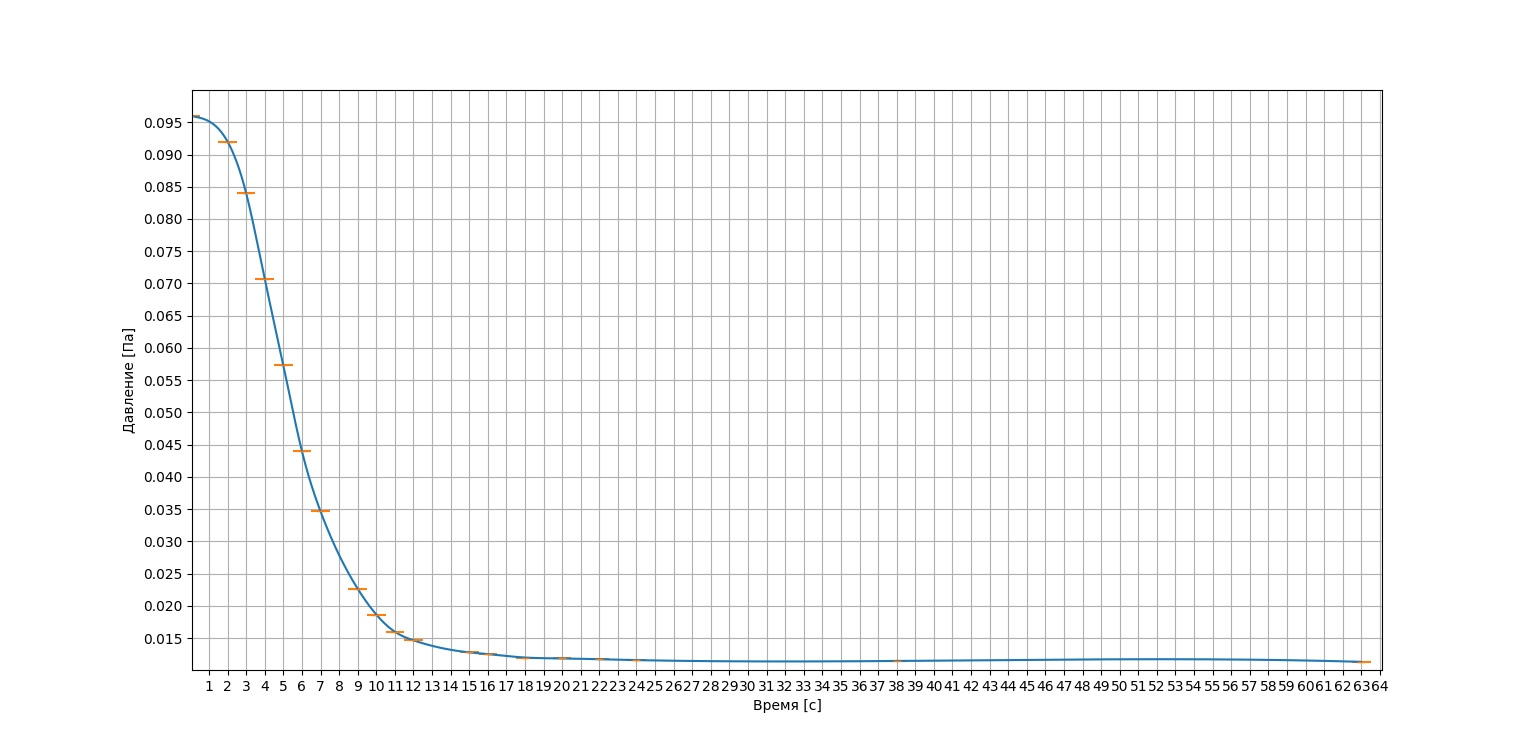
\includegraphics[scale = 0.3]{fig2.jpg} \\
Как видим, зависимость на участке 2-10 секунд напоминает экспоненциальную, что описывается формулой: 
\begin{equation}\label{PbyTime}
P = P_{0}\exp{-\frac{W}{V}\cdot t}+P_{limit}
\end{equation}
\\
, где $P_{0}$ - некотрое начальное значение давления, $W$ - скорость откачки, $P_{limit}$ - предельное значение давления
\\
После учаска экспоненциальной зависимости наблюдаем прямую, практически параллельную оси x. Значит в установке было достигнуто предельное давление, и коэффициент наклона $\alpha \xrightarrow[]{} 0$.

Убедимся в экспоненциальной зависимости на участке 2-10, и рассчитаем скорость откачки $W$. Для этого построим график в логарифмическом масштабе по оси $y$ и методом наименьших квадратов рассчитаем коэффициент наклона прямой:\\
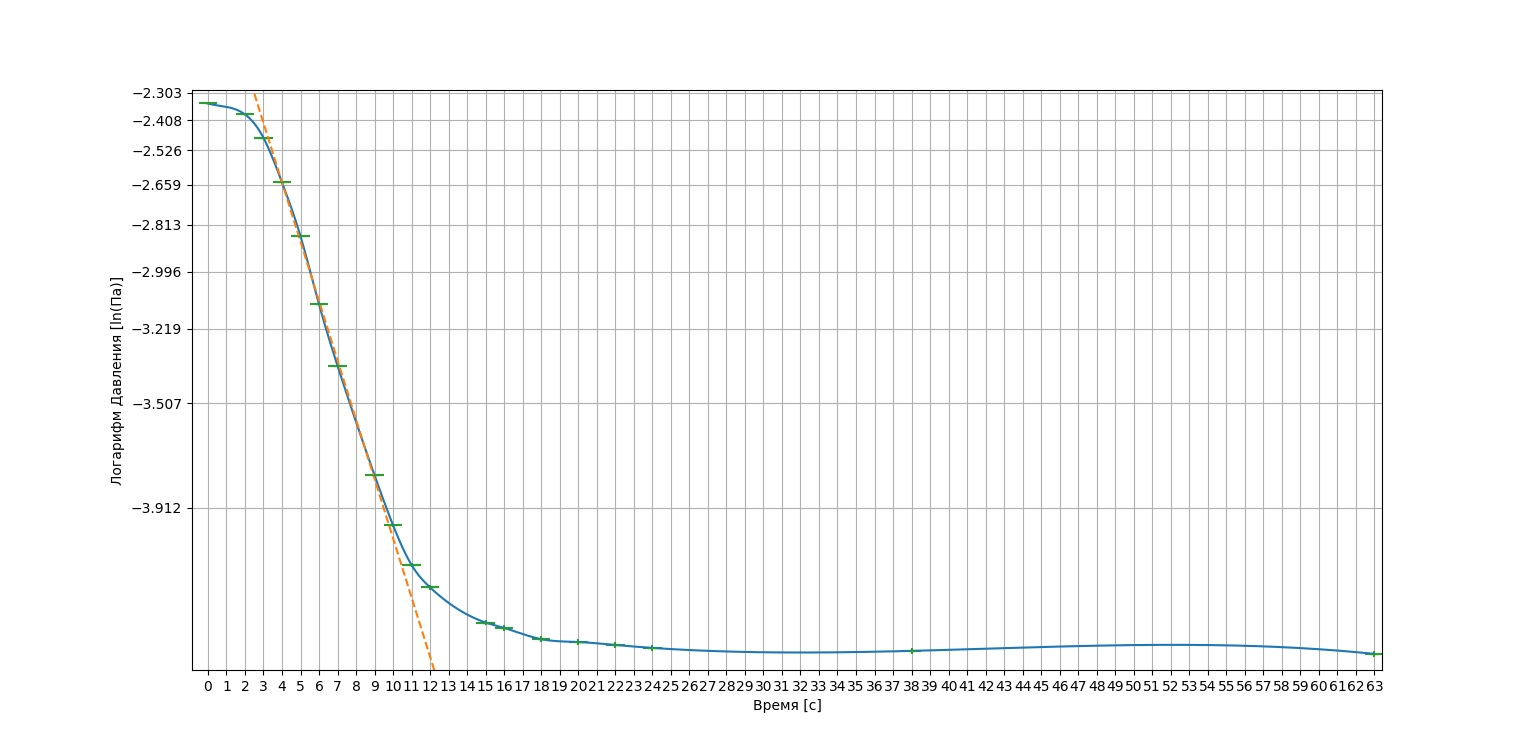
\includegraphics[scale = 0.3]{fig3.jpg}
\begin{equation}
\alpha = -0.230 \pm 0.005
\end{equation}
Выразим сокрость откачки из формулы \eqref{PbyTime}:
\begin{equation}\label{difflnP}
    d\ln{P} = -\frac{W}{V}\cdot dt
\end{equation}
\begin{equation}\label{W}
    W = -\alpha V
\end{equation}
Получим $W = 0.80 \pm 0.04$ л/c
\subsection{Рассчитаем поток газа, поступающего из насоса в откачивающую систему}

Теперь потсроим график зависимости давления от времени при ухудшении вакуума, методом наименьших квадратов оценим коэффициенты наклона:
\begin{equation}
    \alpha = 1.09 \cdot 10^{-3} \pm 1 \cdot 10^{-5}
\end{equation}
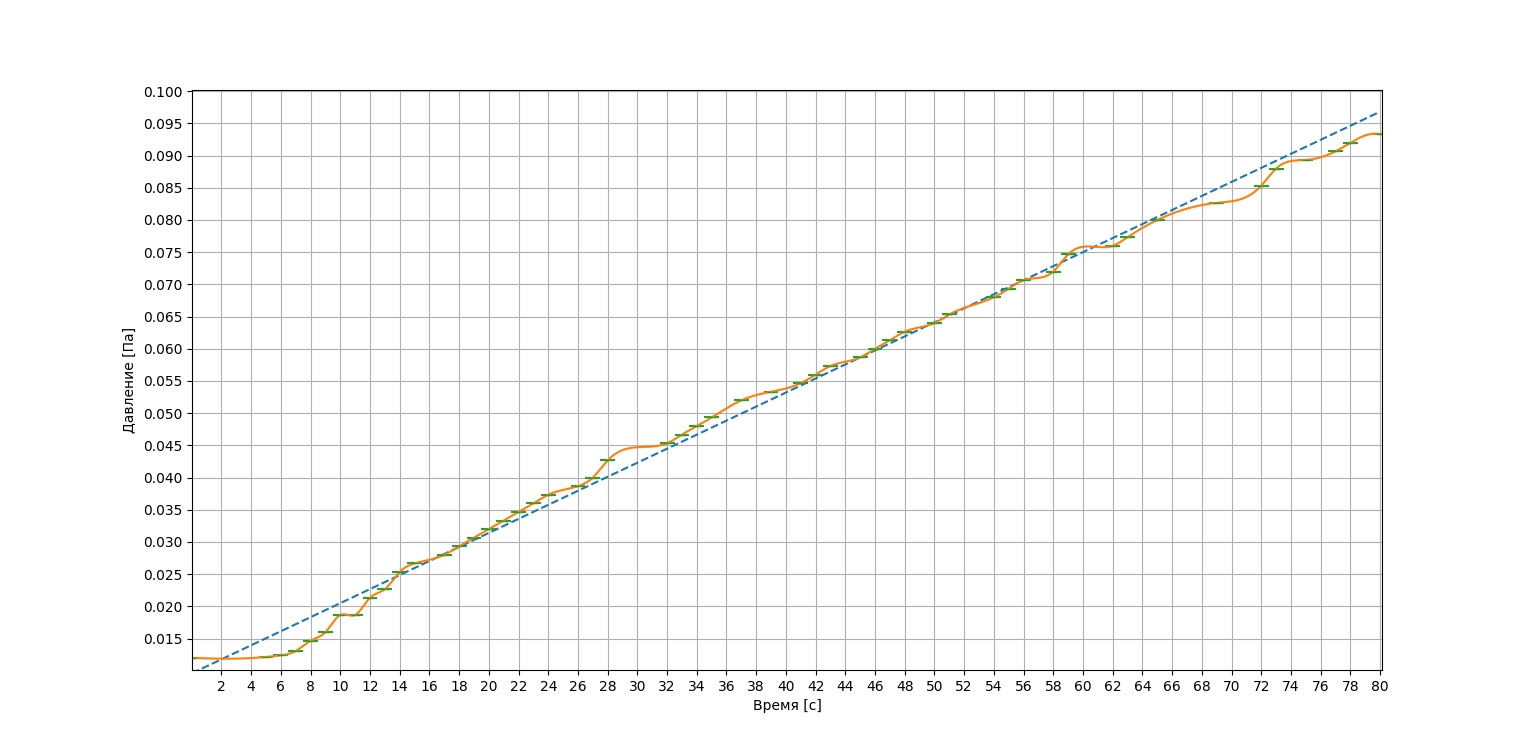
\includegraphics[scale = 0.3]{fig1.jpg}

Воспользуемся основным уравнением, описывающим процесс откачки. Учтем, что во время выполнения данной части эксперемента течей извне создано не было: $Q_{out} = 0$. Получим:
\begin{equation}
    Q_{p} = P_{limit}W - V_{hv} \alpha
\end{equation}
Методом частных производных оценим погешности, в результате получим значение:
$Q_{p} = 0.0073 \pm 0.0005$ Л*Па/с
\subsection{Измерение скорости откачки в условиях течи}


Воспользуемся формулами:
\begin{equation}
    P_{limit} W = Q_{1} 
\end{equation}
\begin{equation}
    P_{set} W = Q_{1}+\frac{d (P V)_{k}}{d t}
\end{equation}
Выразим $Q_{1}$ - сумму натеканий без учета натекания через искусственную течь. Подставив выраженное значение в формулу (6) и рассчитав количество газа, проходящего через каппиляр сможем рассчитать скорость откачки.В результате получим: $W_{1} = 0.0560 \pm 0.0012$ л/с. 
\section{Вывод}
С точностью $5 \%$ удалось рассчитать скорость откачки. Скорость откачки во втором эксперименте меньше скорости откачки в первом примерно на $25 \%$. Очевидно, так как искусственная течь 'мешает' откачке. Об аккуратности проведения эксперимента и правильной работе оборудования можно судить по малому коэффициенту наклона графика зависимости $P(t)$ в эксперименте по ухудшению вакуума и малая масса газа потсупающая в установку через насос. Предельное давление, полученное в эксперименте, составило порядка $8.3 \cdot 10^{-5}$ мм.рт.с, что соответсвует длине свободного пробега порядка нескольких дециметров. Такой вакуум классифицируется как <<высокий>>, так как равновероятно столкновение со стенками и с другими молекулами: $\lambda/d \approx 1$.


\end{document}